\documentclass[a4paper,10pt,twoside]{report}

% Packages for enhancing LaTeX capabilities
\usepackage[a4paper, inner=4cm, outer=3cm, top=2.5cm, bottom=2.5cm]{geometry}
\usepackage{fontspec}
\usepackage{setspace}
\usepackage{fancyhdr}
\usepackage{graphicx}
\usepackage[backend=biber,style=apa]{biblatex}
\usepackage{csquotes}
\usepackage[ngerman]{babel}
\usepackage{float}
\usepackage{amsmath}



\setmainfont{Arial}
\setstretch{1.2}
\pagenumbering{roman}
\setcounter{page}{1}
\addbibresource{../../Ressourcen/Bibliographie/ba_literatur.bib}


\begin{document}

% Titlepage
\begin{titlepage}
  \hspace*{\fill}
  
\includegraphics[width=0.4\textwidth,keepaspectratio]{../../Ressourcen/Bilder/FHE-AI_Logo.png}

  \centering
  \vspace*{1cm}

  \vspace{0.5cm}

  {\Huge\textbf{Bachelorarbeit in der Angewandten Informatik}}
  \\
  Registriernummer: AI-2024-BA-030

  \vspace{1.5cm}

  {\large\textbf{Konzeption und Entwicklung einer datenbankseitigen Abbildung von frei definierbaren Bilanzräumen
      im Zusammenhang mit dem Energiemanagementsystem EMS-EDM PROPHET® nach ISO 50001.}}

  \vspace{1.5cm}

  {\Large\textbf{Fabian Heinlein}}
  \\ in Kooperation mit dem Fraunhofer Institut Angewandte Systemtechnik (IOSB-AST)

  \vspace{1cm}

  \Large Abgabedatum: 28.02.2024

  \vspace{1cm}

  Prof. Dr. Marcel Spehr \\
  Sven Möller

  \vfill

\end{titlepage}



\chapter*{Kurzfassung}
\addcontentsline{toc}{chapter}{Kurzfassung}
\chapter*{Abstract}
\addcontentsline{toc}{chapter}{Abstract}
\chapter*{Vorwort}
\addcontentsline{toc}{chapter}{Vorwort}
\tableofcontents

%%%%%%%%%%%%%%%%%%%%%%%%%% Einleitung %%%%%%%%%%%%%%%%%%%%%%%%%%
\chapter{Einleitung}
\pagenumbering{arabic}
\setcounter{page}{1}

\section{Hintergrund und Motivation}
Angesichts wachsender Umweltbelastungen und der Notwendigkeit nachhaltiger Praktiken spielt das Energiemanagement eine immer bedeutendere Rolle.
Diese Arbeit untersucht die Entwicklung einer datenbankseitigen Lösung zur Abbildung frei definierbarer Bilanzräume im Energiemanagementsystem
EMS-EDM PROPHET® nach DIN EN ISO 50001:2018-12.
Sie wird durch das Potenzial, bei der Verbesserung der energiebezogenen Leistung und Energieeffizienz von Organisationen im tertiären Wirtschaftssektor 
durch die Erfüllung ausgewählter Kriterien der DIN EN ISO 50001:2018-12 zu unterstützen, motiviert. 
Bilanzräume stellen das zentrale Konzept der Arbeit dar und werden im Rahmen dieser als Einheiten betrachtet, die zur digitalen Abbildung 
von Organisationsstrukturen im Energiemanagement und als administrative Grenze zur Bilanzierungsrechnung dienen.
Die Adressierung der Arbeit auf die freie definierbare Gestaltung der Bilanzräume soll eine Möglichkeit bieten, der Diversität von Organisationen innerhalb des 
tertiären Wirtschaftssektors gerecht zu werden
und einen Einsatz der Forschungsergebnisse in solchen Organisationen mit dem EDM-EMS-Prophet® ermöglichen.
Die Untersuchung soll zur Weiterentwicklung nachhaltiger Energiemanagementpraktiken beitragen und Einblicke in die Integration
technischer Lösungen in bestehende Systeme bieten.

Ein wesentlicher Fokus dieser Arbeit liegt auf der DIN EN ISO 50001:2018-12, einer Norm der Internationalen Organisation für Normung (ISO),
die Anforderungen an Energiemanagementsysteme festlegt. Diese Norm ist universell einsetzbar, unabhängig von Größe, Art oder Standort der Organisation (\cite[S. 10]{DIN50001.2018}),
und dient der fortlaufenden Verbesserung der energiebezogenen Leistung. (\cite[S. 7]{DIN50001.2018}).
Um die Anforderungen der DIN EN ISO 50001:2018-12 zu erfüllen, müssen Organisationen den kontinuierlichen Fortschritt ihrer energiebezogenen Leistung nachweisen, wobei
die Norm keine spezifischen Zielniveaus vorgibt. (\cite[S. 10]{DIN50001.2018}).

Die Umsetzung der DIN EN ISO 50001:2018-12 in Organisationen bringt sowohl operationale als auch organisatorische Herausforderungen mit sich [S. 11](\cite{Marimon.2017}).
Dennoch lag im Jahr 2023 in 24.924 Organisationen weltweit ein Zertifikat nach DIN EN ISO 50001:2018-12 vor (\cite{InternationalOrganizationforStandardization.2023}).
Dies ist bemerkenswert, da die Erfüllung der Normanforderungen voraussichtlich etwa 60 \% des globalen Energieverbrauchs beeinflussen
kann (\cite{InternationalOrganizationforStandardization.2011}, zitiert nach \cite[S. 1]{Marimon.2017}). Darüber hinaus entstehen für Organisationen durch
die Einführung der Norm signifikante Vorteile.

Zum einen können nach Aussagen der DIN EN ISO 50001:2018-12 (2018, S. 9) ökonomische Vorteile wie Energieeinsparungen erzielt werden, wodurch Organisationen einen Wettbewerbsvorteil
aufgrund sinkender Energiekosten erlangen können. Zum anderen ergeben sich operationale Vorteile wie eine gesteigerte Produktivität, verbesserte Qualität
und ein strukturierter Ansatz zur Prozessoptimierung (\cite{Marimon.2017}). Des Weiteren kann die Umsetzung der DIN EN ISO 50001:2018-12 dazu beitragen, die allgemeinen
Klimaschutzziele zu erreichen (\cite{DIN50001.2018}). Dies unterstreicht die gesellschaftliche Bedeutung der Norm, insbesondere angesichts der Herausforderungen
des Klimawandels.

Die Umsetzung der DIN EN ISO 50001:2018-12 basiert auf dem PDCA-Zyklus (Plan, Do, Check, Act), der Organisationen einen strukturierten Rahmen für die fortlaufende
Verbesserung der energiebezogenen Leistung bieten soll (\cite[S. 7f.]{DIN50001.2018}).
Während die Norm in erster Linie Anforderungen auf Managementebene formuliert, verweist sie auch auf technische Normen wie die E DIN ISO 50006:2024-07, die unter anderem
spezifische Anforderungen an Energieleistungskennzahlen und energetische Ausgangsbasen definiert (\cite{DIN50006.2024,DIN50001.2018}).


\section{Problemstellung}
\subsection{Problembeschreibung}
\textbf{Forschungsfrage:} "Welche strukturellen Erweiterungen und Anpassungen müssen auf Datenbankebene in EMS-EDM PROPHET® konzipiert und implementiert 
werden, um eine frei definierbare Abbildung von Bilanzräumen zu ermöglichen, die Organisationen bei der Erfüllung der ISO 50001 unterstützt?"

Die breite Anwendbarkeit der in der DIN EN ISO 50001:2018-12 gestellten Anforderungen auf Organisationen führt zu Anforderungen an die Abbildbarkeit von 
frei definierbaren energiebezogenen Organisationsstrukturen im Energiemanagementsystem.

Ein Teilaspekt zur Umsetzung der DIN EN ISO 50001:2018-12 im Rahmen der Energiebilanzierung ist die Abbildung von energiebezogenen Bereichen in 
Organisationen im Energiemanagementsystem und soll im Rahmen dieser Arbeit betrachtet werden.

Die aktuelle Datenbankstruktur von EMS-EDM Prophet® steht vor dem Problem, frei definierbare Bilanzräume abzubilden.
Um dieses Problem zu lösen, sind strukturelle Änderungen und Erweiterungen der Datenbank notwendig.
Somit besteht das zentrale Problem dieser Arbeit darin, ein System zur Abbildung frei definierbarer Bilanzräume auf Datenbankebene unter Berücksichtigung 
der von der DIN EN ISO 50001:2018-12 gestellten Anforderungen an Bilanzräume und damit verbundene Themenkomplexe in EMS-EDM Prophet® zu konzipieren und 
zu implementieren.

Die Problemlösung umfasst alle Aspekte, die auf Grundlage der Vorgaben der Norm sowie praktischer Gegebenheiten konzipiert und auf Datenbankebene 
umgesetzt werden müssen, um EMS-EDM PROPHET® so zu erweitern, dass das System in der Lage ist, Organisationen bei der Erfüllung der ISO 50001 zu 
unterstützen. Dies gilt insbesondere für Anforderungen, die durch die Abbildung von Bilanzräumen adressiert werden können.

Aufgrund der Anwendbarkeit der DIN EN ISO 50001:2018-12 auf alle Organisationen ist die freie Definierbarkeit der Bilanzräume ein Qualitätskriterium des zu 
entwerfenden Systems und spielt bei der Beantwortung der Forschungsfrage eine zentrale Rolle.
Die breite Anwendbarkeit der Norm impliziert außerdem die Notwendigkeit, praktische Herausforderungen beim Einsatz der Lösung zu berücksichtigen und 
Anwendungsgebiete des entworfenen Konzepts zu betrachten, um der praktischen Relevanz dieser Arbeit gerecht zu werden.

\subsection{Praktische Relevanz des Problemraums} 
Das beschriebene Problem weist eine praktische Relevanz auf, da es die Herausforderungen der DIN EN ISO 50001:2018-12
im Energiemanagement von Organisationen adressiert.
Die bestehenden Anforderungen der DIN EN ISO 50001:2018-12 und der aktuelle Zustand von EMS-EDM Prophet® stellen praxisnahe Qualitätskriterien an die Abbildung von Bilanzräumen.
Eine Herausforderungen besteht darin, ein Datenbankmodell zu entwickeln, das diese Anforderungen erfüllt und gleichzeitig praxisnah und umsetzbar ist.
Die Berücksichtigung von aus der Praxis abgeleiteten Anforderungen ist dabei unerlässlich.
Dies verdeutlicht die Notwendigkeit einer Methodik, die sowohl theoretische als auch praktische Aspekte integriert.
Die Integration der Lösung in EMS-EDM Prophet® stellt sicher, dass sie in bestehenden Organisationen nutzbar ist und deren Energiemanagement unterstützt.

\subsection{Wissenschaftliche Relevanz des Problemraums} 
Die Problemstellung weist eine wissenschaftliche Relevanz auf, da im Zuge der Erarbeitung einer Lösung Methoden des Datenmanagements im Kontext der 
Modellierung von Energiebilanzräumen angewandt werden.
Dabei werden die in EMS-EDM Prophet® bestehenden Methoden um neue Ansätze zur Modellierung von Bilanzräumen erweitert.
Diese Erweiterungen tragen zur wissenschaftlichen Diskussion über Datenmanagementstrategien im Energiemanagement bei und bieten neue Perspektiven für die 
Integration von Bilanzräumen in datenbankbasierte Systeme.
Darüber hinaus fördert die Arbeit den interdisziplinären Austausch zwischen den Bereichen Energiemanagement und Datenbankmodellierung, indem sie 
theoretische Konzepte mit praktischen Anwendungen verknüpft.
Die entwickelten methodischen Ansätze und Modelle können als Grundlage für zukünftige wissenschaftliche Untersuchungen dienen und die Weiterentwicklung 
von Energiemanagementsystemen unterstützen.


\section{Ziel der Arbeit}

Das Ziel dieser Arbeit ist die Konzeption, Implementation und Evaluation eines Prototyps, der durch strukturelle Anpassungen und 
Erweiterungen des EMS-EDM Prophet® die Abbildung frei definierbarer Bilanzräume ermöglicht. Der Prototyp soll einen Mehrwert zur 
Erfüllung der Anforderungen der DIN EN ISO 50001:2018-12 bieten und in Organisationen des tertiären Wirtschaftssektors, die EMS-EDM Prophet® nutzen, 
anwendbar sein. Die Erarbeitung des Prototyps soll auf den theoretischen Grundlagen des Daten- und Energiemanagements basieren und bewährte Ansätze 
aus den Bereichen verwenden. Außerdem soll der Prototyp praktische Herausforderungen in den potentiellen Anwendungsgebieten berücksichtigen und 
allgemeine Anforderungen an Organisationen zu dessen Umsetzung formulieren.


Zur Evaluation des Prototyps soll die Bilanzraumstruktur der Organisation: Fraunhofer IOSB-AST in Ilmenau im entworfenen Prototyp abgebildet werden.
Der angewendete Prototyp soll im Bezug auf die unterstützung bei der Erfüllung der DIN EN ISO 50001:2018-12 Anforderungen auf qualitative und quantitative 
Qualitätskriterien evaluiert werden.
Außerdem soll die freie Definierbarkeit und die praktische Anwendbarkeit des Prototyps evaluiert werden.



\section{Aufbau der Arbeit}
Diese Arbeit ist so konzipiert, dass Sie die theoretischen Grundlagen des Problemraums erfasst und Nutzen sowie Herausforderungen im Anwendungsgebiet: 
EMS nach DIN EN ISO 50001:2018-12 erarbeitet. 
Basierend auf den theoretischen Grundlagen im Anwendungsbereich und den bestehenden Methoden und Ansätzen des Datenmanagements 
in EMS-EDM Prophet® wird eine Lösung der Forschungsfrage auf Datenbankebene des Energiemanagementsystems konzipiert, 
implementiert und evaluiert.
Der Aufbau der Arbeit umfasst drei Hauptabschnitte: die theoretischen Grundlagen und der Stand der Wissenschaft, die Konzeption und Implementation, und die 
Evaluation.

\begin{enumerate}
    \item \textbf{Theoretische Grundlagen und Stand der Wissenschaft}
    
    Die praxisnahe Problemstellung erfordert eine anwendungsorientierte Forschung unter Berücksichtigung der Interdisziplinarität. 
    Im theoretischen Teil der Arbeit werden zwei Themenbereiche betrachtet: Grundlagen der Energiebilanzierung unter Nutzung von Bilanzräumen und  
    Energiemanagementsysteme nach DIN EN ISO 50001:2018-12. In beiden Tehemenbereichen findet die erarbeitung der Grundlagen unter beachtung des Anwendungsgebiets: 
    Organisation im tertiären Wirtschaftssektor statt. 
    
    Für die Erarbeitung der theoretischen Grundlagen des Energiemanagements werden im ersten Hauptabschnitt der Arbeit die DIN EN ISO 50001:2018-12, 
    damit verbundene Normen und Basiswissen aus für den Problemraum relevanter Fachliteratur analysiert.
    Außerdem werden wissenschaftliche Arbeiten aus verwandten Problemräumen analysiert und in den Kontext dieser Arbeit gesetzt.
    Auf dieser Basis werden theoretische Konzepte und Anforderungen aus dem Problemraum abgeleitet, die für die Lösung der Forschungsfrage relevant sind.
    
    Der erste Hauptabschnitt der Arbeit hat somit eine zentrale Bedeutung zum erreichen der Interdisziplinarität der Forschung.
    Die umfangreiche erarbeitung von Konzepten des Energiemanagements, Anforderungen von Anforderungen der ISO 50001 und den Einsatzmöglichkeiten 
    von Bilanzräumen zur praxisnahen erfüllung dieser Anforderungen auf basis der Konzepte stellen eine detaillierte Analyse des Anwendungsbereichs dieser 
    Forschung dar.
    Diese Detaillierte Analyse, ohne technische Perspektive der Datenbankmodellierung, ist notwendig um der Interdisziplinarität des Problemraums aus Sicht des 
    Energiemanagements und der Energiebilanzierung gerecht zu werden. 
    Die erarbeiteten Grundlagen des Anwendungsbereichs: Energiemanagent wird im nächsten Hauptabschnitt, der Konzeption und Implementation, 
    aufgegriffen und aus einer technischen Sicht des Datenbankmanagements betrachtet.

    \item \textbf{Konzeption und Implementation des Prototyps}

    Basierend auf den Forschungsergebnissen des theoretischen Teils der Arbeit wird im zweiten Kapitel der Arbeit eine Lösung für den Problemraum
    konzipiert und implementiert.
    Um der Interdisziplinarität aus Sicht der Datenbankmodellierung gerecht zu werden, wird der IST-Zustand des EMS-EDM Prophet® analysiert und es werden 
    bereits bestehende Ansätze der Datenbankmodellierung die den Problemraum addressieren aufgezeigt.
    Unter berücksichtigung der aufgezeigten Ansätze wird der Prototyp zur Problemlösung konzipiert und EMS-EDM Prophet® im implementiert.
    Im Zuge dessen ist die konzeption und integration von Ansätzen des Datenbankmanagements, die noch nicht im EMS-EDM Prophet® bestehen 
    notwendig.
    Das Konzept addressiert die im ersten Hauptabschnitt erarbeiteten Erkenntnisse des Anwendungsbereichs: Energiemanagement und Energiebilanzierung 
    und stellt eine Datenbankseitige abbildung der Grundsätze unter den erarbeiteten Anforderungen der ISO 50001 im kontext von Organisationen des 
    tertiären Wirtschaftssektors zur verfügung.
    
    \item \textbf{Evalutation des Prototyps}
    
    Im dritten Hauptabschnitt der Arbeit wird der entworfene Prototyp evaluiert.
    Im Zuge dessen wird die Bilanzraumstruktur des Fraunhofer IOSB-AST in Ilmenau erarbeitet und im entworfenen Prototyp abgebildet.
    Anhand dieses praktischen Beispiels wird getestet wie korrekt die im ersten Hauptabschnitt erläuterten Methoden des Energiemanagements und der Energiebilanzierung 
    umgesetzt wurden, und wie der Prototyp in der Praxis bei der Erfüllung von ISO 50001 Anforderungen Organisationen unterstützen kann. 
    Dieser Abschnitt der Evaluation findet unter Nutzung quantitativer Qualitätskriterien statt.

    Des weiteren wird grundsätzlich betrachtet, wie im Rahmen der Interdisziplinarität die im ersten Hauptabschnitt erarbeiteten Erkenntnisse aus Sicht 
    des Energiemanagements technisch durch den konzipierten und implementierten Prototyp abgebildet wurde.
    Dabei wird auch analysiert ob und wie die im ersten Hauptabschnitt erörterten Anforderungen der ISO 50001 auf Datenbankebene umgesetzt wurden sind.
    Dieser Abschnitt der Evaluation findet unter Nutzung qualitativer Qualitätskriterien statt.

\end{enumerate}


%%%%%%%%%%%%%%%%%%%%%%%%%% Theoretische Grundlagen %%%%%%%%%%%%%%%%%%%%%%%%%%

\chapter{Stand der Forschung und Theoretische Grundlagen}
\section{Grundlagen von Bilanzräumen}
\subsection{Bilanzierung}

%%%%%%%%%%%%%%%%%%%%%%%%%%%%%%%%%%%%%%%%%%%%%%%%%%%%%%%%%%%%%%%%%%%%%%%%%%%%%%%%%%%%%%%%%%%%%%%%%%%%%%%%%%%%%%%%%%%%%%%%%%%%%%%%%%%%%%%%%%%%%%%%%%%%%%%%%%%%%%%%%%%
\subsubsection{Kontext der Bilanzierung}

Bilanzierung ist ein Konzept welches in unterschiedlichen Einsatzbereichen verwendung findet. Diese Forschung befasst sich mit Bilanzräumen 
im Kontext der DIN EN ISO 50001:2018-12. Die Norm setzt den Schwerpunkt auf die fortlaufende Verbesserung der energiebezogenen Leistung 
(\cite[Kapitel 0.2]{DIN50001.2018}). Aufgrund dessen sollte die Bilanzierung in diesem Forschungskontext aus einer Perspektive betrachtet werden welche 
energiebezogene Größen betrachtet.

Auch die Festlegung auf Organisationen des tertiären Wirtschaftssektors hat auswirkungen auf die betrachtungsweise der Bilanzierung. 
Denn in Organisation mit immateriellen Dienstleistungen spielt die Gebäudeenergie eine vorrangige Rolle zur Verbesserung der energiebezogenen 
Leistung (\cite[S. 3]{Fichera.2020}). 
Dies lässt sich Beispielhaft an der Abbildung \eqref{fig:Energieverbrauch_Wärme_DE} darstellen.

\begin{figure}[H]
    \centering
    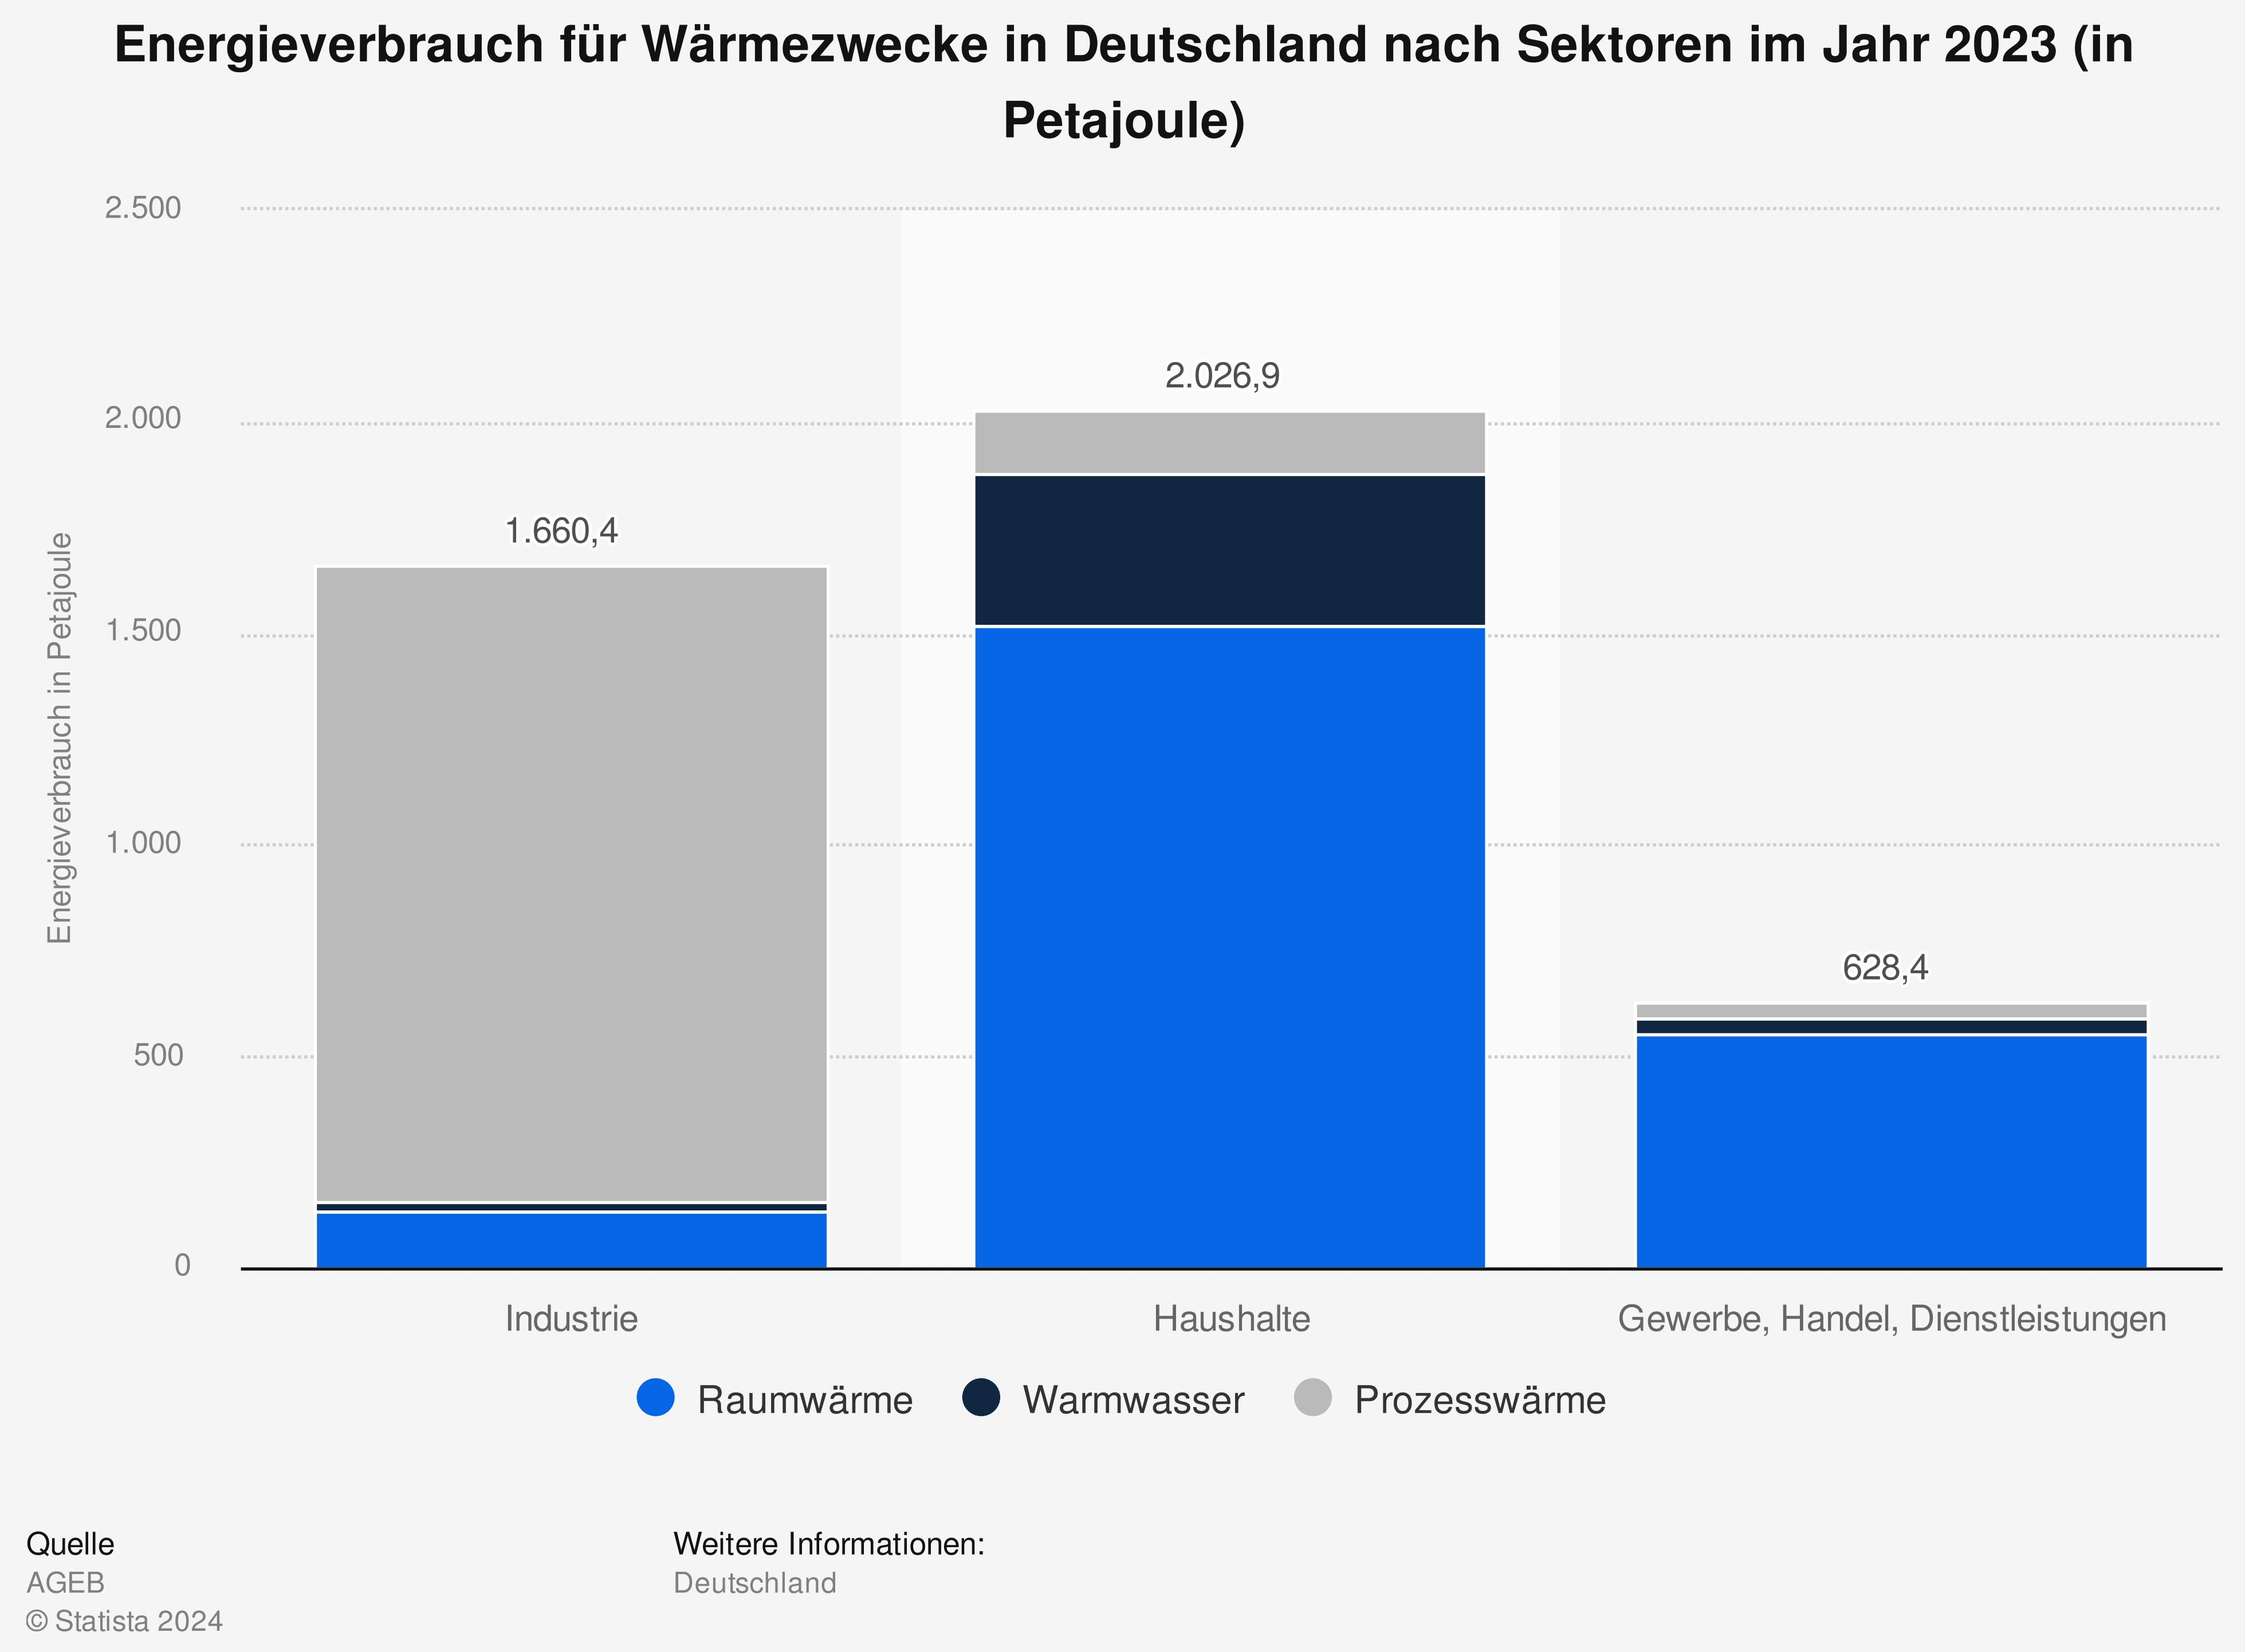
\includegraphics[width=0.68\textwidth]{../../Ressourcen/Bilder/Energieverbrauch_für_Wärmezweck_DE.jpg}
    \caption{Energieverbrauch für den Wärmezweck in Deutschland [\cite{AGEB.2024}]}
    \label{fig:Energieverbrauch_Wärme_DE}
\end{figure}

Die Abbildung \ref{fig:Energieverbrauch_Wärme_DE} zeigt den Energieverbrauch für Wärmezwecke in Deutschland im Jahr 2023, aufgeschlüsselt nach Sektoren. 
Während der industrielle Sektor einen hohen Anteil an prozessbezogener Wärme aufweist, spielt im Dienstleistungssektor die Raumwärme 
eine dominante Rolle.
Diese Statistik bekräftigt die Aussage von Fichera (2020, S. 3) dass bei der Verbesserung der energiebezogenen Leistung in Organisationen des tertiären 
Wirtschaftssektors energiebezogene Prozesse und Technologien im Gegensatz zur Gebäudeenergie eine untergeordnete Bedeutung haben. 

Im Rahmen der Bestimmung des Gesamtenergiebedarfs eines Gebäudes über den Lebenszyklus wird vor allem der Gebäudebetrieb betrachtet (\cite[S. 133]{Musall.2015}).
Die sogenannte Graue Energie wird üblicherweise als kumulierter, nicht erneuerbarer Primärenergieaufwand beschrieben, der alle vor- und nachgelagerten 
Prozesse der verwendeten Baustoffe und Materialien sowie der technischen Anlagen umfasst (\cite[S. 133]{Musall.2015}). Da die DIN EN ISO 50001:2018-12 
auf die fortlaufende Verbesserung der energiebezogenen Leistung abzielt und die Graue Energie konstant ist wird diese im Rahmen dieser Arbeit nicht 
betrachtet. 
Stattdessen liegt der Fokus dieser Forschungsarbeit auf der Bilanzierung energetischer Größen im Rahmen von Organisation des tertiäten Wirtschaftssektors. 
Sie grenzt sich somit von der Bilanzierung von Rohstoffen und Materialien ab.

%%%%%%%%%%%%%%%%%%%%%%%%%%%%%%%%%%%%%%%%%%%%%%%%%%%%%%%%%%%%%%%%%%%%%%%%%%%%%%%%%%%%%%%%%%%%%%%%%%%%%%%%%%%%%%%%%%%%%%%%%%%%%%%%%%%%%%%%%%%%%%%%%%%%%%%%%%%%%%%%%%%

\subsubsection{Definition Bilanzierung}
Im Rahmen des beschrieben Kontexts rückt die verfahrenstechnische Perspektive der Bilanzierung in den Fokus. 
So wird die Bilanzierung im Kontext der Verfahrenstechnik nach Rönsch (2015, S. 66) in drei Bilanzgleichungen unterteilt: 
die Massenbilanz, die Energiebilanz und die Impulsbilanz. 
Zur Beantwortung dieser Forschungsfrage hat insbesondere die Energiebilanz eine hohe Relevanz.

Die Energiebilanz beruht auf dem Energieerhaltungssatz (\cite[S. 66]{Rönsch.2015}), der das Prinzip der Erhaltung 
der Energie ausdrückt (\cite[S. 57]{Baehr.1966}). Der Energieerhaltungssatz bezieht sich auf alle Erscheinungsformen, in denen Energie auftritt, 
und besagt, dass es unmöglich ist, Energie zu erzeugen oder zu vernichten (\cite[S. 57]{Baehr.1966}). 
Für zu bilanzierende Systeme bedeutet dies, dass die Energie in einem abgeschlossenen, adiabaten System über die Zeit 
konstant ist (\cite[S. 66]{Rönsch.2015}). 
Adiabat bedeutet in diesem Kontext, dass das System keine Wärme mit seiner Umgebung austauscht (\cite[S. 66]{Rönsch.2015}). 

Für Systeme, die in der Lage sind, Energie zu speichern, impliziert dies nach Rönsch (2015, S. 66f.), 
dass die darin gespeicherte Energie gleich der Differenz aus ein- und austretenden Energieströmen ist. 
Für offene, nicht-adiabate Systeme ohne Speicherfähigkeit gilt, dass die Differenz der ein- und austretenden Energieströme Null ist 
(\cite[S. 66f.]{Rönsch.2015}).
Das von Rönsch (2015, S. 66f.) beschriebene Verhalten eines Systems bezüglich der Energiespeicherung, lässt sich mathematisch 
vereinfacht mit der Gleichung \eqref{energiebilanzierungsgleichung_Rönsch} darstellen:

\begin{equation}
E_{\text{gespeichert}} = \sum E_{\text{eingang}} - \sum E_{\text{ausgang}}
\label{energiebilanzierungsgleichung_Rönsch}
\end{equation}

\begin{description}
    \item \(E_{\text{gespeichert}}\): Im System gespeicherte Energie.
    \item \(E_{\text{eingang}}\): Energie eines eintretenden Energiestroms.
    \item \(E_{\text{ausgang}}\): Energie eines austretenden Energiestroms.
    \item Für offene, nicht-adiabate Systeme ohne Energiespeicher gilt:
    \[
    E_{\text{gespeichert}} = 0
    \]
    \item In diesem Fall ist die zugeführte Energie gleich der abgegebenen Energie:
    \[
    \sum E_{\text{eingang}} = \sum E_{\text{ausgang}}
    \]
\end{description}

Diese Gleichung beschreibt einen allgemeinen Ansatz zur Energiebilanzierung der im System gespeicherten Energie. 
Im Rahmen der Bilanzierung komplexer Systeme kann jedoch eine detailliertere Bilanzierung einzelner Zustandsgrößen im System erforderlich sein.

Dieses Problem wird von der von Ahrendts (2014, Kapitel 1.5) aufgestellten Bilanzgleichung im Kontext der Thermodynamik addressiert. 
Die Gleichung basiert auf dem Fakt, dass sich für jede mengenartige Zustandsgröße, die über die Grenze eines Systems transportiert wird, eine 
Bilanz aufstellen lässt (\cite[Kapitel 1.5]{Ahrendts.2014}). 
Diese Bilanz umfasst ein- und austretende Ströme sowie im System enthaltene Energiequellen und -senken und ermittelt die 
Geschwindigkeit der Änderung des Bestands der zu bilanzierenden Zustandsgröße im System (\cite[Kapitel 1.5]{Ahrendts.2014}).

Die von Ahrendts (2014, Kapitel 1.5) aufgestellte Bilanzgleichung wird in den Formeln \eqref{BilanzierungsgleichungAhrendt} und 
\eqref{BilanzierungsgleichungAhrendtStrom} dargestellt.

\begin{equation}
    dX_{\text{j}}/d\tau = (\sum \dot{X}_{\text{j,e}} - \sum \dot{X}_{\text{j,a}}) + (\dot{X}_{\text{j,Quell}} - \dot{X}_{\text{j,Senk}})
    \label{BilanzierungsgleichungAhrendt}
\end{equation}

\begin{description}
    \item \(X_{\text{j}}\): Zustandsgröße.
    \item \(\tau\): Zeitintervall.
    \item \(X_{\text{j,e}}\): Über die Systemgrenze zufließende Zustandsgröße.
    \item \(X_{\text{j,a}}\): Über die Systemgrenze abfließende Zustandsgröße.
    \item \(X_{\text{j,Quell}}\): Quellen der Zustandsgröße im System.
    \item \(X_{\text{j,Senk}}\): Senken der Zustandsgröße im System.
\end{description}

Im Rahmen der Formel \eqref{BilanzierungsgleichungAhrendt} wird der Strom einer Zustandsgröße \(X_{\text{j}}\) in Gleichung 
\eqref{BilanzierungsgleichungAhrendtStrom} definiert.

\begin{equation}
    \dot{X}_{\text{j}} = \lim_{\Delta\tau \to 0} \Delta X_{\text{j}}/ \Delta\tau
    \label{BilanzierungsgleichungAhrendtStrom}
\end{equation}

\begin{description}
    \item \(X_{\text{j}}\): Zustandsgröße.
    \item \(\Delta X_{\text{j}}\): Menge der Größe \(X_{\text{j}}\) im Zeitintervall \(\Delta \tau\).
    \item \(\Delta \tau\): Zeitintervall.
\end{description}

Die Gleichung \eqref{BilanzierungsgleichungAhrendt} in Verbindung mit \eqref{BilanzierungsgleichungAhrendtStrom} beschreibt die Geschwindigkeit 
der Änderung des Bestands der Größe \(X_{\text{j}}\) als Summe der Differenzen zwischen den über die Systemgrenze zu- und abfließenden Strömen der 
Zustandsgröße \(X_{\text{j}}\) sowie den Quell- und Senkströmen der Zustandsgröße \(X_{\text{j}}\) innerhalb des Systems.  
Somit formulieren die Gleichungen \eqref{energiebilanzierungsgleichung_Rönsch} und \eqref{BilanzierungsgleichungAhrendt} in Verbindung mit 
\eqref{BilanzierungsgleichungAhrendtStrom} eine grundlegende und zugleich vereinfachte mathematische Beschreibung einer Bilanzierung im Kontext 
der Thermodynamik und Verfahrenstechnik. Sie bilden die Basis für die Beschreibung der grundlegenden Struktur einer Bilanz.
Im Folgenden werden die in \eqref{energiebilanzierungsgleichung_Rönsch} und \eqref{BilanzierungsgleichungAhrendt} mit \eqref{BilanzierungsgleichungAhrendtStrom} 
beschriebenen Bestandteile einer Bilanz zur Konzeption eines Bilanzraums im Anwendungskontext des Problemraums analysiert. 


\subsection{Bilanzräume in der Energiewirtschaft}

%%%%%%%%%%%%%%%%%%%%%%%%%%%%%%%%%%%%%%%%%%%%%%%%%%%%%%%%%%%%%%%%%%%%%%%%%%%%%%%%%%%%%%%%%%%%%%%%%%%%%%%%%%%%%%%%%%%%%%%%%%%%%%%%%%%%%%%%%%%%%%%%%%%%%%%%%%%%%%%%%%%

\subsubsection{Bilanzraumgrenzen zur Abbildung des bilanzierten Systems}
Eine Bilanz bezieht sich gemäß Ahrendts (2014, Kapitel 1.5) auf das von der Systemgrenze eingeschlossene Kontrollgebiet. 
Die Systemgrenze kann dabei unter Berücksichtigung der Zweckmäßigkeit frei definiert werden (\cite[Kapitel 1.5]{Ahrendts.2014}).
Das definierte System kann auch als Bilanzraum bezeichnet werden, da die Berechnung der in einen Bilanzraum ein- und austretenden Ströme als Bilanzierung bezeichnet wird (\cite[S. 65]{Rönsch.2015}).
Einen Ansatz zur Definition von Bilanzräumen liefert Miller (2016, S. 105) mit der Konkretisierung von Bewertungsräumen mittels Kriterien der Bilanzgrenze, dem 
Aggregationsniveau und der Bewertungseinheit. Das definierte System Dient der Bewertung der Nutzung der Ressourcen wobei der Effizienzbegriff eine zentrale Rolle spielt (\cite[S. 107]{Miller.2016}).
Miller (2016, S. 107) definiert die Effizienz nach Gleichung \eqref{EffizienzgleichungMiller}.

\begin{equation}
    \text{Effizienz} := \frac{\text{Erreichter Nutzen}}{\text{Aufwand}}
    \label{EffizienzgleichungMiller}
\end{equation}

Der Aufwand umfasst nach Miller (2016, S. 108f.) unterschiedliche Ressourcen, wobei im Kontext energiewirtschaftlicher Fragestellungen der Fokus auf der Ressource Energie 
liegt.
Der Nutzen ist vom Untersuchungsgegenstand abhängig und wird im Kontext der energiewirtschaftlichen 
Fragestellung häufig über Energiedienstleitstungen operationalisiert (\cite[S. 107]{Miller.2016}). Betrachtet man dass der Nutzen grundsätzlich durch Befriedigung 
von Bedürfnissen beschrieben wird entsteht im Kontext der Energiewirtschaft ein Nutzenergiebedarf zur Befriedigung der Bedürfnisse im Rahmen einer Energiedienstleitstung 
(\cite[S. 107]{Miller.2016}). 
Sowohl die Ressourcen des Aufwands als auch die Energiedienstleistung auf Nutzenseite werden durch eine Bewertungseinheit formalisiert (\cite{Miller.2016}).
Der Nutzen wird meist implizit durch den gewählten Untersuchungsgegenstand definiert (\cite[S. 110]{Miller.2016}).
Die in \eqref{EffizienzgleichungMiller} aufgestellte Nutzen-Aufwand Relation stellt die Grundlage der Definition der Bilanzraumgrenze dar. 
Die Bilanzraumgrenze lässt sich somit in die Aufwandsseitige Bilanzgrenze, die alle zu bilanzierenden Ressourcen umfasst und die Nutzenseitige Bilanzrgrenze die sich auf 
die zu Bilanzierende Energiedienstleitstung bezieht (\cite[S. 111]{Miller.2016}).  

Das von Miller (2016) beschriebene Konzept bringt eine neue Perspektive auf die in \eqref{BilanzierungsgleichungAhrendt} und \eqref{BilanzierungsgleichungAhrendtStrom} 
aufgestellte Bilanzgleichung. Sie bringt das Prinzip der Effizienz ein und teilt eine Bilanz in Aufwands und Nutzenseite. 
Aufwandsseitig sind die in \eqref{BilanzierungsgleichungAhrendt} zufließenden Ströme, also die dem System zugeführten Ressourcen der Zustandsgröße zu betrachten. 
Nutzenseitig müssen abfließende Ströme, also die aus dem System fließende Energie zur Befriedigung der Energiedienstleistung der Zustandsgröße betrachtet werden. 
Die abfließenden Ströme werden nach Energiedienstleistung mit Nutzengrößen operationalisiert (\cite{Miller.2016}).

%%%%%%%%%%%%%%%%%%%%%%%%%%%%%%%%%%%%%%%%%%%%%%%%%%%%%%%%%%%%%%%%%%%%%%%%%%%%%%%%%%%%%%%%%%%%%%%%%%%%%%%%%%%%%%%%%%%%%%%%%%%%%%%%%%%%%%%%%%%%%%%%%%%%%%%%%%%%%%%%%%%

\subsubsection{Zustandsgrößen, Nutzengrößen und Nutzenergiebedarf}
In einem Thermodynamischen System wird der augenblickliche Zustand durch die Zustandsgrößen beschrieben, wobei diese in intensive und extensive Zustandsgrößen 
unterschieden werden (\cite[S. 66]{Konstantin.2023}). Die innere Energie U ist eine extensive Zustandsgröße (\cite[S. 65]{Konstantin.2023}), und rückt in den 
Fokus da es sich um eine energetische Zustandsgröße handelt. Das Verhalten einer Zustandsgröße ist in \eqref{BilanzierungsgleichungAhrendt} und \eqref{BilanzierungsgleichungAhrendtStrom} 
beschrieben.

In dieser Forschung bezieht sich der Untersuchungsgegenstand aufgrund der verortung der Organisationen im tetriären Wirtschaftssektors auf Gebäudeenergie. 
Es müssen also auf der Grundlage dieses Untersuchungsgegenstands angemessene Nutzengrößen mit entsprechenden Bewertungseinheiten erfasst werden. 
Da auch die Definition der Systemgrenze vom Untersuchungsgegenstand beeinflusst wird (\cite[S. 109]{Miller.2016}) gilt die Zweckmäßigkeit der Systemgrenze 
auch für die zu untersuchenden Nutzengrößen.
Die DIN EN ISO 50001:2018-12 gibt mit dem Ziel der fortlaufenden Verbesserung der energiebezogenen Leistung eine Vorgabe zur zweckmäßigen Definition der Nutzengröße 
(\cite[S. 11]{DIN50001.2018}).
Die Vornorm DIN V 18599-1:2018-09, herausgegeben vom Deutschen Institut für Normung e. V. (2018, S. 1), behandelt die energetische Bewertung von Gebäuden und stellt ein 
Verfahren zur Durchführung der Gesamtenergiebilanz bereit (\cite[S. 9]{DIN18599.2018}). Ihre Ausrichtung auf die energetische Bewertung erfüllt die Zweckmäßigkeit der 
DIN EN ISO 50001:2018-12. Der Fokus auf die Bewertung von Gebäuden entspricht der Zielsetzung der DIN V 18599-1:2018-09. 

Im Rahmen der energetischen bewertung von Gebäuden betrachtet die DIN V 18599-1:2018-09 die Bilanzierung des Nutz-, End- und Primärenergiebedarf (\cite{DIN18599.2018}).
In einem energiewirtschaftlichen Rahmen hat besonders der Nutzeenergiebedarf eine Große Bedeutung da er aus der Befriedigung der Bedürfnisse im Rahmen einer 
Energiedienstleistung resultiert (\cite[S. 107]{Miller.2016}).

\begin{figure}[H]
    \centering
    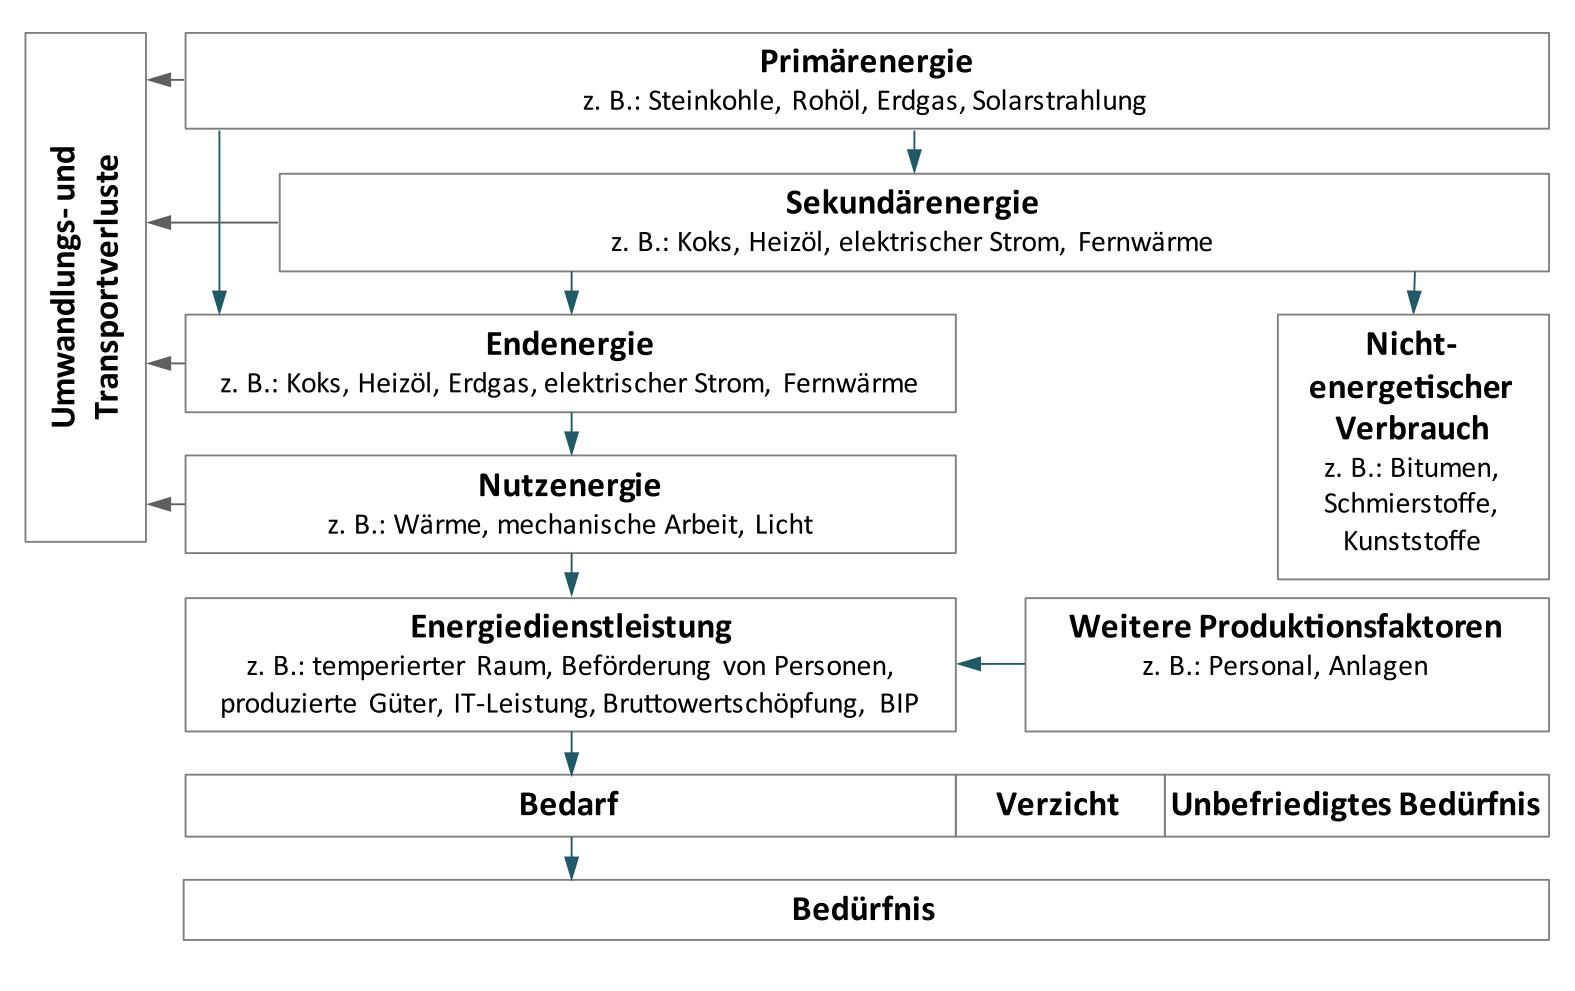
\includegraphics[width=0.8\textwidth]{../../Ressourcen/Abbildungen/Energiefluss_Miller.jpg}
    \caption{Energieflussschema. (Dargestellt von Miller (2016))}
    \label{fig:Energieflussschema_Miller}
\end{figure}

Im Energieflussdiagramm \eqref{fig:Energieflussschema_Miller} wird die Nutzenergie zwischen der Endenergie und der Energiedienstleistungen verortet. 
Da die Endenergie die Energiemenge ist, die dem Bilanzraum zur bestimmungsgemäßen Nutzung bereitgestellt wird (\cite[Kapitel 3.1.2]{DIN18599.2018}), 
Repräsentiert diese Energieform die Menge der potentiellen Ressourcen auf Aufwandsseite der Bilanzierung.
Außerdem wird der praktische Sachverhalt veranschaulicht dass bei der Umwandlung von Endenergie in Energiedienstleistungen über die Nutzenergie 
Umwandlungs und Transportverluste berücksichtigt werden müssen.

Die DIN V 18599-1:2018-09 definiert die Heizung, Kühlung, Lüftung, Trinkwarmwasseraufbereitung und Beleuchtung von Gebäuden oder Gebäudezonen 
als relevante Nutzengrößen zur energetischen Bewertung von Gebäuden (\cite{DIN18599.2018}). 
Somit wird im von Miller (2016) aufgestellten Konzept der Nutzenergiebedarf der jeweiligen Nutzengröße durch die Nutzenergie gedeckt, 
und muss je nach Nutzengröße unterschiedlich definiert werden. Die Nutzenergie wird im Konzept von Miller (2016) durch die Ressourcen repräsentiert.
Im Rahmen der Vornorm wird der Nutzenergiebedarf als Überbegriff für Nutzwärmebedarf, Nutzkältebedarf, Nutzenergiebedarf für Tinkwarmwasser, Beleuchtung und 
Befeuchtung definiert (\cite[Kapitel 3.1.3]{DIN18599.2018}).
Der Nutzenergiebedarf der Beleuchtung ist definiert als rechnerisch ermittelter Energiebedarf, der sich ergibt, wenn die Gebäudezone mit der im Nutzungsprofil 
festgelegten Beleuchtungsqualität beleuchtet wird (\cite[Kapitel 3.1.6]{DIN18599.2018}). 
Analog dazu versteht sich die Nutzeenergie für die Beleuchtung als die Energiemenge die zur Ausreichenden Beleuchtung der Gebäudezone aufgewendet werden muss (\cite[Kapitel 5.3.1]{DIN18599.2018}).
Der Nutzwärmebedarf hingegen ist der rechnerisch ermittelter Wärmebedarf, der zur Aufrechterhaltung der festgelegten thermischen Raumkonditionen innerhalb einer Gebäudezone während der Heizzeit benötigt wird
rechnerisch ermittelter Energiebedarf, der sich ergibt, wenn die Gebäudezone mit der im Nutzungsprofil festgelegten Beleuchtungsqualität beleuchtet wird(\cite[Kapitel 3.1.4]{DIN18599.2018}).
Der Nutzkältebedarf ist der rechnerisch ermittelter Kühlbedarf, der zur Aufrechterhaltung der festgelegten thermischen Raumkonditionen innerhalb einer Gebäudezone benötigt wird in Zeiten, 
in denen die Wärmequellen eine höhere Energiemenge anbieten als benötigt wird(\cite[Kapitel 3.1.5]{DIN18599.2018}).
Die Wärmeenergie ist die Wämemenge, die der Gebäudezone zusätzlich (bedarfs-)geregelt zugeführt werden muss, um die vorgegebene 
Sollinnentemperatur einzuhalten (\cite[Kapitel 5.3.1]{DIN18599.2018}).
Der Nutzenergiebedarf für die Trinkwarmwasserbereitung ist definiert als der rechnerisch ermittelte Kühlbedarf, der zur Aufrechterhaltung der festgelegten thermischen Raumkonditionen innerhalb einer Gebäudezone benötigt wird in Zeiten, in denen die Wärmequellen eine höhere Energiemenge anbieten als benötigt wird
rechnerisch ermittelter Energiebedarf, der sich ergibt, wenn die Gebäudezone mit der im Nutzungsprofil festgelegten Menge an Trinkwarmwasser entsprechender Zulauftemperatur versorgt wird (\cite[Kapitel 3.1.7]{DIN18599.2018}).
Die Nutzenergie für die Trinkwarmwasserbereitung bedeutet die Energiemenge für die Erwärmung des Trinkwassers von der Kaltwassertemperatur auf die 
Warmwassertemperatur an der Entnahmestelle (\cite[Kapitel 5.3.1]{DIN18599.2018}).
Im Rahmen der Luftaufbereitung versteht sich die Nutzenergie als Energiemenge die zum Erwärmen, Kühlen, Befeuchten und Entfeuchten der Luft in einer 
raumlufttechnischen Anlage zu- beziehungsweise abgeführt werden muss um den erforderlichen Zuluftzustand zu erreichen (\cite[Kapitel 5.3.1]{DIN18599.2018}).

Abbildung \eqref{fig:Übersicht_Bilanzräume} Ordnet den mithilfe der DIN V 18599-1:2018-09 erfassten Untersuchungsgegenstand in das von Miller (2016) erarbeitete Konzept der 
Bewertungsräume ein.

\begin{figure}[H]
    \centering
    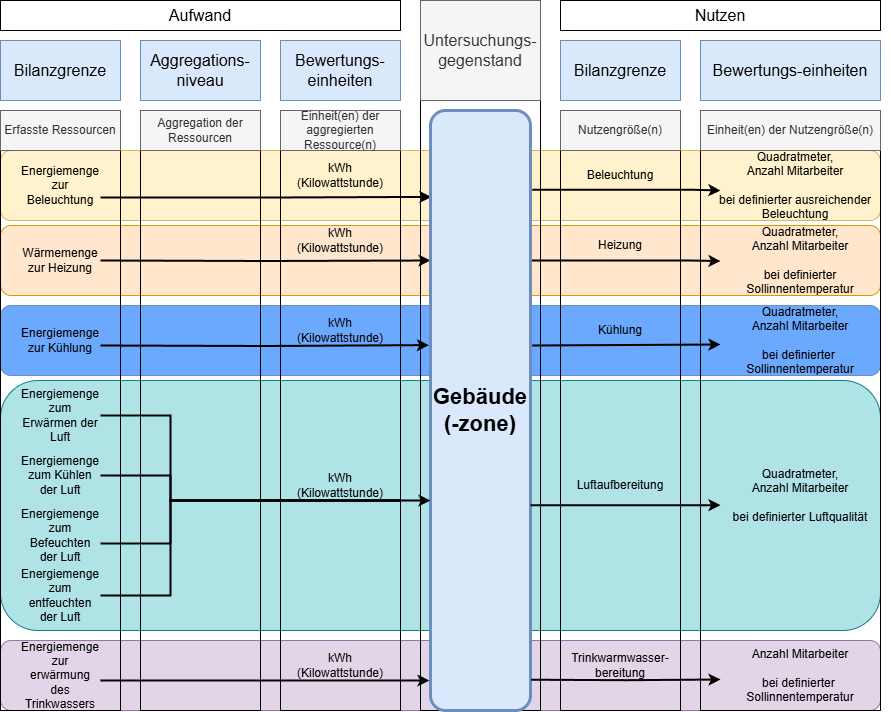
\includegraphics[width=1\textwidth]{../../Ressourcen/Abbildungen/Nutzengröße_Bewertungseinheit.png}
    \caption{Übersicht Bilanzräume. (Eigene Darstellung basierend auf Miller (2016) und DIN V 18599-1:2018-09 (2018))}
    \label{fig:Übersicht_Bilanzräume}
\end{figure}

%%%%%%%%%%%%%%%%%%%%%%%%%%%%%%%%%%%%%%%%%%%%%%%%%%%%%%%%%%%%%%%%%%%%%%%%%%%%%%%%%%%%%%%%%%%%%%%%%%%%%%%%%%%%%%%%%%%%%%%%%%%%%%%%%%%%%%%%%%%%%%%%%%%%%%%%%%%%%%%%%%%

\subsubsection{Energieströme und Bewertungseinheiten}
In der Gleichung \eqref{BilanzierungsgleichungAhrendtStrom} wird der Strom einer Zustandsgröße als Menge der Zustandsgröße in einem infinitesimal kleinen Zeit-
intervall definiert, welches im Grenzwert gegen 0 geht. Folglich wird ein Strom von Ahrendts (2014) als Menge einer Zustandsgröße zu einem bestimmten Zeitpunkt 
definiert. 

In Gleichung \eqref{BilanzierungsgleichungAhrendt} wird zwischen in das System zu- und abfließende Ströme der Zustandsgröße Unterschieden.
Die zufließenden Ströme können als Ressourcen der Aufwandsseite im von Miller (2016) aufgestellten Konzept der Bewertungsräume betrachtet werden, 
wobei energetische Ressourcen im Vordergrund stehen. Aufwandsseitige Ressourcen können zu einer Ressource mit einer Bewertungseinheit 
zusammengefasst werden (\cite[S. 112]{Miller.2016}). Sollten nach erfassung und optionaler aggregation der Ressourcen mehrere Ressourcenkategorien bestehen, 
können diese mit unterschiedlichen Bewertungseinheiten bilanziert werden (\cite[S. 112]{Miller.2016}). Im Rahmen dieser Forschungsarbeit werden 
Aufwandsseitig jedoch ausschließlich Energieressourcen betrachtet.
Sie Stammen somit aus dem Bereich der Endenergie und haben die Bewertungseinheit: kWh und deren Vielfaches da diese Einheit bei Energiebilanzen in der Regel für alle 
Energieformen bevorzugt verwendet wird (\cite[S. 65]{Konstantin.2023}).

Die abfließenden Ströme in \eqref{BilanzierungsgleichungAhrendt} repräsentieren die Nutzenseite des von Miller (2016) aufgestellten Konzepts.
Um die Nutzenseite abzubilden ist eine Konkretisierung der Energiedienstleistung durch eine angemessene Bewertungseinheit, 
welche vom Untersuchungsgegenstände impliziert wird notwendig (\cite{Miller.2016}). Diese Bewertungseinheit ist keine Energieeinheit, und 
kann beispielsweise bei der Untersuchung der Temperierung von Räumen die Quadratmeteranzahl des Bilanzraums bei einer definierten 
soll Temperierung sein (\cite{Miller.2016}). 

Eine praktische Herausforderung im Rahmen der Bilanzierung ist die Energiedatensammlung der zu erfassenden Ströme zu der auch die DIN EN ISO 50001:2018-12 vorgaben macht. 
Die DIN EN ISO 50001:2018-12 (2018, Kapitel 6.6, A.6.6) stellt Anforderungen und Qualitätskriterien an die Datensammlung in Organisationen.
Diese verpflichtet Organisationen dazu Hauptmerkmale ihrer Tätigkeiten, die sich auf die energiebezogene Leistung auswirken zu identifizieren, und diese in geplanten 
Zeitabständen zu messen, überwachen und analysieren (\cite[S. 23]{DIN50001.2018}).
Teil der zu erfassenden Hauptmerkmale sind relevante Variablen bezüglich wesentlicher Energieeinsätze, den Energieverbrauch bezüglich wesentlicher Einsätze 
und der Organisation und betriebliche Kriterien bezüglich wesentlicher Energieeinsätze(\cite[S. 23]{DIN50001.2018}).
Die komplexität der Umsetzung ist dabei nicht vorgeschrieben und kann von einfachen Zählwerten bis hin zu umfangreichen Werten aus Überwachungs- und Messystemen mit 
Softwareandwendung reichen (\cite[S. 36]{DIN50001.2018}).

%%%%%%%%%%%%%%%%%%%%%%%%%%%%%%%%%%%%%%%%%%%%%%%%%%%%%%%%%%%%%%%%%%%%%%%%%%%%%%%%%%%%%%%%%%%%%%%%%%%%%%%%%%%%%%%%%%%%%%%%%%%%%%%%%%%%%%%%%%%%%%%%%%%%%%%%%%%%%%%%%%%

\subsubsection{Energiequellen und -senken}
Gleichung \eqref{BilanzierungsgleichungAhrendt} unterscheidet zwischen Quellen, Senken und zu- beziehungsweise abfließenden Strömen der Zustandsgröße. 
Quell- und Senkenströme treten in einer Energiebilanz nach dem ersten Hauptsatz der Thermodynamik nicht auf da Energie als Erhaltungsgröße ist (\cite[S. 14]{Ahrendts.2014}). 
Im Rahmen der DIN EN ISO 50001:2018-12 bezieht sich der Begriff Energie auf verschiedene Arten von Energie die erworben, gespeichert, aufbereitet, in einer Einrichtung oder einem Prozess verwendet 
oder zurückgewonnen werden können (\cite[Kapitel 3.5.1]{DIN50001.2018}). Energie kann im Rahmen der Norm als Elektrizität, Brennstoff, Dampf, Wärme, Druckluft oder vergleichbares Medium auftreten 
(\cite[Kapitel 3.5.1]{DIN50001.2018}).
Folglich werden alle Energieströme, in denen Energie in eine Energieform umgewandelt wird, die nicht die genannten Kirterien erfüllen als Energiesenken betrachtet. 
Analog dazu werden alle Energieströme, bei denen Energie, die nicht den von der Norm aufgestellten Kriterien entspricht, in eine nach ISO 50001 definierte Energieform 
umgewandelt wird, als Energiequellen betrachtet.
In der Praxis stellen die in Abbildung \eqref{fig:Energieflussschema_Miller} dargestellten Umwandlungs- und Transportverluste Energiesenken dar. Energiequellen können beispielsweise 
PV-Anlagen sein, da diese die Energie des Sonnenlichts, welche nach Definition der DIN EN ISO 50001:2018-12 nicht Nutzbar ist in nutzbare Energie umwandelt und als 
Endenergie zur Verfügung steht.

\subsubsection{Bilanzraumstrukturen}
Bisher wurde die strukturelle Definition von Bilanzräumen unter anbetracht praktischer Herausforderung unter der DIN EN ISO 50001:2018-12 in Organisationen 
des tertiären Wirtschaftssektors betrachtet. Allerdings können auch zwischen Bilanzräumen Beziehungen bestehen, welche im folgenden erläutert werden.

Ein Bilanzraum kann in mehrere Teilbilanzräume zerlegt werden (\cite[S. 310]{Engelmann.2015}). Dies kann durch die Zerlegung in einzelne Prozesse, 
Anlagen oder Räumlich getrennte Bereiche realisiert werden (\cite[S. 310]{Engelmann.2015}), wobei die Zerlegung in Prozesse bei Organisationen des tertiären 
Wirtschaftssektors eine geringere Relevanz hat.
Analog zur Zerlegbarkeit eines Bilanzraums lässt sich auch der Untersuchungsgegenstand eines Bilanzraums Hierarchisch aufgliedern (\cite[S. 109]{Miller.2016}).

Zur Erfassung der Energiedaten einer Organisation bedarf es eine detaillierte und aussagekräftige Analyse der Unterscheidung nach Verbrauchsarten 
(\cite[S. 14]{Hohnhold.2013}). Dabei ist die Disagggregation der Daten von der Größe der Organisation und dem Zweck der Analyse möglich (\cite[S. 14f.]{Hohnhold.2013}).
Die beschriebene Unterscheidung nach Verbrauchsarten kann durch die Zerlegung eines Bilanzraums mit mehreren Nutzengrößen in Bilanzräume mit einer Nutzengröße 
realisiert werden. Da die DIN V 18599-1:2018-09 Gebäude in Zonen, welche als grundlegende räumliche Berechnungseinheit für die Energiebilanzierung definiert sind (\cite[Kapitel 3.1.12]{DIN18599.2018}), 
unterteilt, ist auch eine Zerlegung des Untersuchungsgegenstands in einzelne Gebäudezonen Sinnvoll.
\subsection{Bilanzraumstrukturen}

\section{Bilanzräume im Energiemanagement nach ISO 50001}


\subsection{Abbildung des Organisationskontext}

\subsection{Identifikation wesentlicher Energieeinsätze}

\subsubsection{Analyse und Unterscheidung von Energieeinsätzen}

Die DIN EN ISO 50001:2018-12 verpflichtet Organisationen im Rahmen der Planungsphase des PDCA-Zyklus zur Identifikation von wesentlichen Energieeinsätzen auf Grundlage 
der vorher durchgeführten Datenanalyse (\cite[S. 25]{DIN50001.2018}).
Die Norm definiert einen Energieeinsatz als Anwendung von Energie zum Beispiel für Energiedienstleistungen wie Lüftung oder Heizung, und bezeichnet den Begriff mitunter als 
Endnutzung von Energie (\cite[Kapitel 3.5.4]{DIN50001.2018}). 
Der Energieeinsatz ergibt sich aus dem Produkt des spezifischen Energieeinsatzes und der Menge der Nachgefragten Energiedienstleistungen (vgl. Gleichung \eqref{EnergieeinsatzMiller}) (\cite[S. 120]{Miller.2016}).
Der Spezifische Energieeinsatz ergibt sich aus dem Kehrwert der Energieeffizienz (vgl. Gleichung \eqref{EffizienzgleichungMiller}) (\cite[S. 120]{Miller.2016}).
\begin{equation}
    \text{Energieeinsatz} := \text{Spezifischer Energieeinsatz} \cdot \text{Menge Energiedienstleistung}
    \label{EnergieeinsatzMiller}
\end{equation}

\begin{equation}
    \text{Spezifischer Energieeinsatz} :=\frac{\text{Aufwand}}{\text{Erreichter Nutzen}}
    \label{SepzifischerEnergieinsatzMiller}
\end{equation}

Betrachtet man beispielsweise eine Heizungsanlage als nutzenseitige Energiedienstleistung im Untersuchungsgegenstand Gebäudezone.
So könnte man den erreichten Nutzen mit der Grundfläche konkretisieren. 
Der Aufwand wird durch den im Bilanzzeitraum anfallenden Nutzenergiebedarf zur befriedigung der Energiedienstleistung: Heizung gemessen.
Der Spezifische Energieeinsatz ist somit der im Bilanzzeitraum entstandene Nutzenergiebedarf zum Heizen pro Quadratmeter. 

Ein wesentlicher Energieeinsatz, auch SEU (en: significant energy use), wird von der Norm als Energieeinsatz der wesentlichen Anteil am Energieverbrauch 
hat und/oder erhebliches Potential für eine Verbesserung der energiebezogenen Leistung bietet definiert (\cite[Kapitel 3.5.6]{DIN50001.2018}). 
SEUs können Anlagen beziehungsweise Standorte, Systeme, Prozesse oder eine Einrichtungen sein (\cite[Kapitel 3.5.6]{DIN50001.2018}).
Zur Definition von Kriterien zur Identifikation von SEUs macht die Norm keine Angaben und verpflichtet die Organisation die die Norm anwendet zur Entscheidung was 
als wesentlicher Energieeinsatz anzusehen ist (\cite[S. 38]{DIN50001.2018}). 
Neben Energieerzeugungsanlagen und Umwandlungsanlagen gibt es Anlagenkategorien für Klimatisierungsanlagen, 
Lüftungsanlagen, Bleuchtungsanlagen sowie Informations- und Kommunikationstechnik (\cite[S. 14]{Hohnhold.2013}).

Eine differenzierte Darstellung der Verbrauchsstrukturen nach Anlagenkategorien beziehungsweise einzelner Anlagen ermöglicht das identifizieren von 
wesentlichen Energieeinsätzen und liefert somit auch Ansatzpunkte zur Verbesserung der Energieeffizienz (\cite{Fink.1997} zitiert nach \cite[S. 8]{Hohnhold.2013}).
Die in Abbildung \eqref{fig:Disagggregation_Bilanzraum_Nutzengrößen} dargestellte Disaggregation eines Bilanzraums nach Nutzengrößen kann bei der Analyse der 
Verbrauchsstrukturen innerhalb eines Untersuchungsgegenstands im Rahmen der Datenanalyse beitragen.



Abbildung \eqref{fig:Disagggregation_Bilanzraum_Nutzengrößen_Beispiel} zeigt Beispielhaft wie die Disagggregation von Bilanzräumen zur Identifikation von 
wesentlichen Energieeinsätzen beitragen kann. 
Der durch die aufwandsseitigen Ressourcen gedeckte Nutzenergiebedarf der bilanzierten Energiedienstleistung kann als absolute Energieleistungskennzahl zur 
Bewertung des Energieeinsatzes für die Energiedienstleistung betrachtet werden.
Der Energieeinsatz kann mit der durch die Bewertungseinheit quantifizierten Energiedienstleistung in relation gesetzt werden um den Spezifischen Energieeinsatz 
(vgl. Gleichung \eqref{SepzifischerEnergieinsatzMiller}) zu ermitteln, welcher als Beziehungszahl kategorisiert werden kann und somit geeignet zur Bewertung der Energieeffizienz ist. 
Die Integration einer Gliederungszahl als EnPI welche den Energieeinsatz eines Bilanzraums einer Energiedienstleistungen in Relation 
zum Energieeinsatz eines Bilanzraums aller Energiedienstleistungen setzt kann (vgl. Gleichung \eqref{Anteil_Gesamtenergieverbrauch}) den Vergleich des Anteils einzeln Energiedienstleistungen 
am Gesamtenergieverbrauch unterstützen.


\begin{equation}
    \text{Anteil Gesamtenergieverbrauch} :=\frac{\text{Energieverbrauch Bilanzraum}}{\text{Gesamtenergieverbrauch}}
    \label{Anteil_Gesamtenergieverbrauch}
\end{equation}

In diesem Beispiel macht die Heizungsanlage des Hauptgebäudes mit einem Energieeinsatz von 18.750 kWh 62,5 \% des Gesamtenergieverbrauchs aus und hat somit einen 
wesentlich Größeren Anteil am Gesamtenergieverbrauch als die Kühlungsanlage des Hauptgebäudes, welche mit einem Energieeinsatz von 3.750 kWh nur 12,5 \% des 
Gesamtenergieverbrauchs ausmacht.
Mit \( 125 \,\frac{\text{kWh}}{\text{m}^2} \) hat die Heizung den höchsten spezifischen Energieeinsatz und somit die geringst Energieeffizienz und die Kühlung 
mit \( 25 \,\frac{\text{kWh}}{\text{m}^2} \) den geringsten spezifischen Energieeinsatz und somit die höchste Energieeffizienz.

\begin{figure}[H]
    \centering
    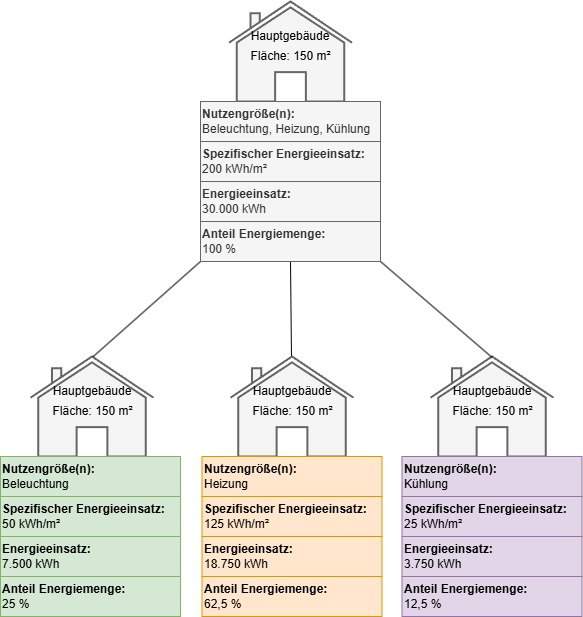
\includegraphics[width=0.7\textwidth]{../../Ressourcen/Abbildungen/Nutzengröße_Bewertungseinheit_Zerlegt_Beispiel.jpg}
    \caption{Beispiel: Disaggregation nach Nutzengrößen. (Eigene Darstellung)}
    \label{fig:Disagggregation_Bilanzraum_Nutzengrößen_Beispiel}
\end{figure}


Eine Analyse der Gebäudezonen innerhalb eines Gebäudes durch Disagggregation nach Untersuchungsgegenstand wie sie in 
\eqref{fig:Disagggregation_Bilanzraum_Untersuchungsgegenstand} visualisiert ist kann zur Identifikation wesentlicher Energieeinsätze durch die Analyse und Unterscheidung 
von Energieeinsätzen innerhalb von Gebäude(-zonen) beitragen.



Abbildung \eqref{fig:Disagggregation_Bilanzraum_Untersuchungsgegenstand_Beispiel} visualisiert beispielhaft, wie eine Disagggregation des Untersuchungsgegenstands 
zur Analyse und Unterscheidung von Energieeinsätzen innerhalb eines Untersuchungsgegenstands beitragen kann.
Zur Bewertung der einzelnen Bilanzräume werden die selben Energieleistungskennzahlen wie in Abbildung \eqref{fig:Disagggregation_Bilanzraum_Nutzengrößen_Beispiel} 
genutzt, allerdings wird der Bilanzraum anhand des Untersuchungsgegenstands disaggregiert.
In diesem Beispiel macht die Gebäudezone 2 mit einem Energieeinsatz von 18.000 kWh 60\% des Gesamtenergieverbrauchs des Gebäudes aus während Gebäudezone 3 mit 
einem Energieeinsatz von 3.000 kWh nur 10\% des Gesamtenergieverbrauchs ausmacht.
Der spezifische Energieeinsatz ist in Gebäudezone 2 mit  \( 300 \,\frac{\text{kWh}}{\text{m}^2} \) am höchsten und somit ist die Energieeffizienz am geringsten. 
In Gebäudezone 3 ist mit \( 100 \,\frac{\text{kWh}}{\text{m}^2} \) der spezifische Energieeinsatz am niedrigsten und die Energieeffizienz somit am höchsten.



\begin{figure}[H]
    \centering
    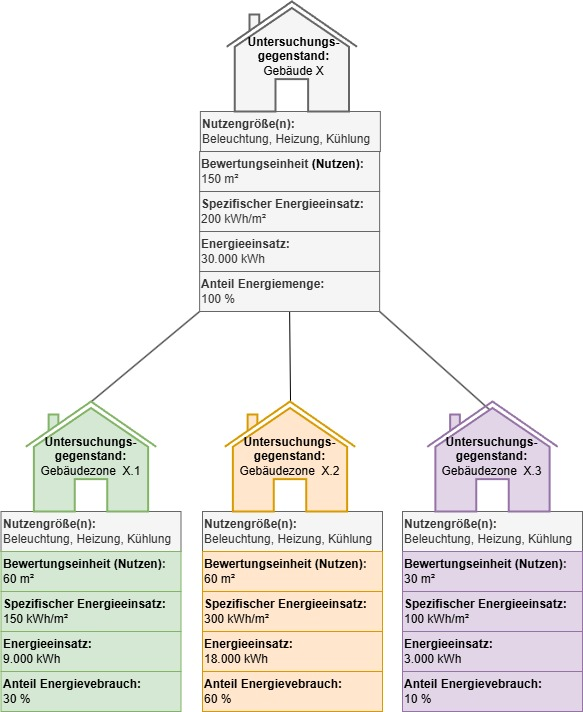
\includegraphics[width=0.7\textwidth]{../../Ressourcen/Abbildungen/Untersuchungsgegenstand_Zerlegt_Beispiel.jpg}
    \caption{Beispiel: Disaggregation nach Untersuchungsgegenstand. (Eigene Darstellung)}
    \label{fig:Disagggregation_Bilanzraum_Untersuchungsgegenstand_Beispiel}
\end{figure}

\subsection{Energieleistungskennzahlen}



%%%%%%%%%%%%%%%%%%%%%%%%%% Konzept %%%%%%%%%%%%%%%%%%%%%%%%%%

\chapter{Konzeption und implementation in EMS-EDM Prophet®}
\section{Einleitung}

\section{Ausgangszustand: EMS-EDM Prophet®}

\section{Anforderungen}
\subsection{Modellierung von Bilanzräumen}

\subsection{Abbildung von Metriken zur Bewertung von Bilanzräumen}

\subsection{Technische Anforderungen und Datenkommunikation}


\section{Umsetzungskonzept für EMS-EDM Prophet®}

\subsection{Systemarchitektur}
\subsection{Datenmodell und Datenbankdesign}
\subsection{Technische Umsetzung und Datenkommunikation}
\subsection{EnPI Abbildung}
\subsection{Test- und Validierungskonzept}
\subsection{Sicherheitskonzept}
\subsection{Bedingungen und Anforderungen an die Laufzeitumgebung}

\section{Technische Realisierung}
In diesem Kapitel sollen alle technischen Aspekte der Umsetzung beschrieben werden.
\section{Umsetzungsablauf}
In diesem Kapitel soll der Ablauf der Umsetzung beschrieben und begründet werden.
\section{Ergebnis}
In diesem Kapitel soll das Ergebnis der Umsetzung beschrieben werden.
\subsection{Anforderungsumsetzung}
In diesem Kapitel soll beschrieben werden wie die Anforderungen umgesetzt wurden und welche Anforderungen umgesetzt wurden.
\subsection{Vergleich zum bestehenden System}
In diesem Kapitel soll der Vergleich zum bestehenden System gezogen werden und erläutert werden was sich verändert hat.


%%%%%%%%%%%%%%%%%%%%%%%%%% Implementation und Evaluation %%%%%%%%%%%%%%%%%%%%%%%%%%

\chapter{Evaluation}

\section{Einleitung}
\subsection{Ziel der Evaluation}
\subsection{Methodik}

\section{Metriken und Kennzahlen}
\subsection{Definition der Erfolgsmessung}
\subsection{Quantitative Metriken}
\subsection{Qualitative Metriken}

\section{Experimenteller Aufbau}
\subsection{Beschreibung des Experimentes}
\subsection{Testumgebung und -bedingungen}
\subsection{Datensätze und Szenarien}

\section{Durchführung und Ergebnisse}
\subsection{Durchführung}
\subsection{Quantitative Ergebnisse}
\subsection{Qualitative Ergebnisse}

\section{Vergleich mit alternativen Ansätzen}

\section{Diskussion der Ergebnisse}

\section{Zusammenfassung der Evaluation}

\chapter{Fazit}
\section{Zusammenfassung der Ergebnisse}
\section{Ausblick auf zukünftige Arbeiten}

\printbibliography[title={Literaturverzeichnis}]

\appendix
\chapter{Anhang}
\section*{Selbstständigkeitserklärung}

\end{document}
